\begin{figure*}[ht]
  \centering
  % 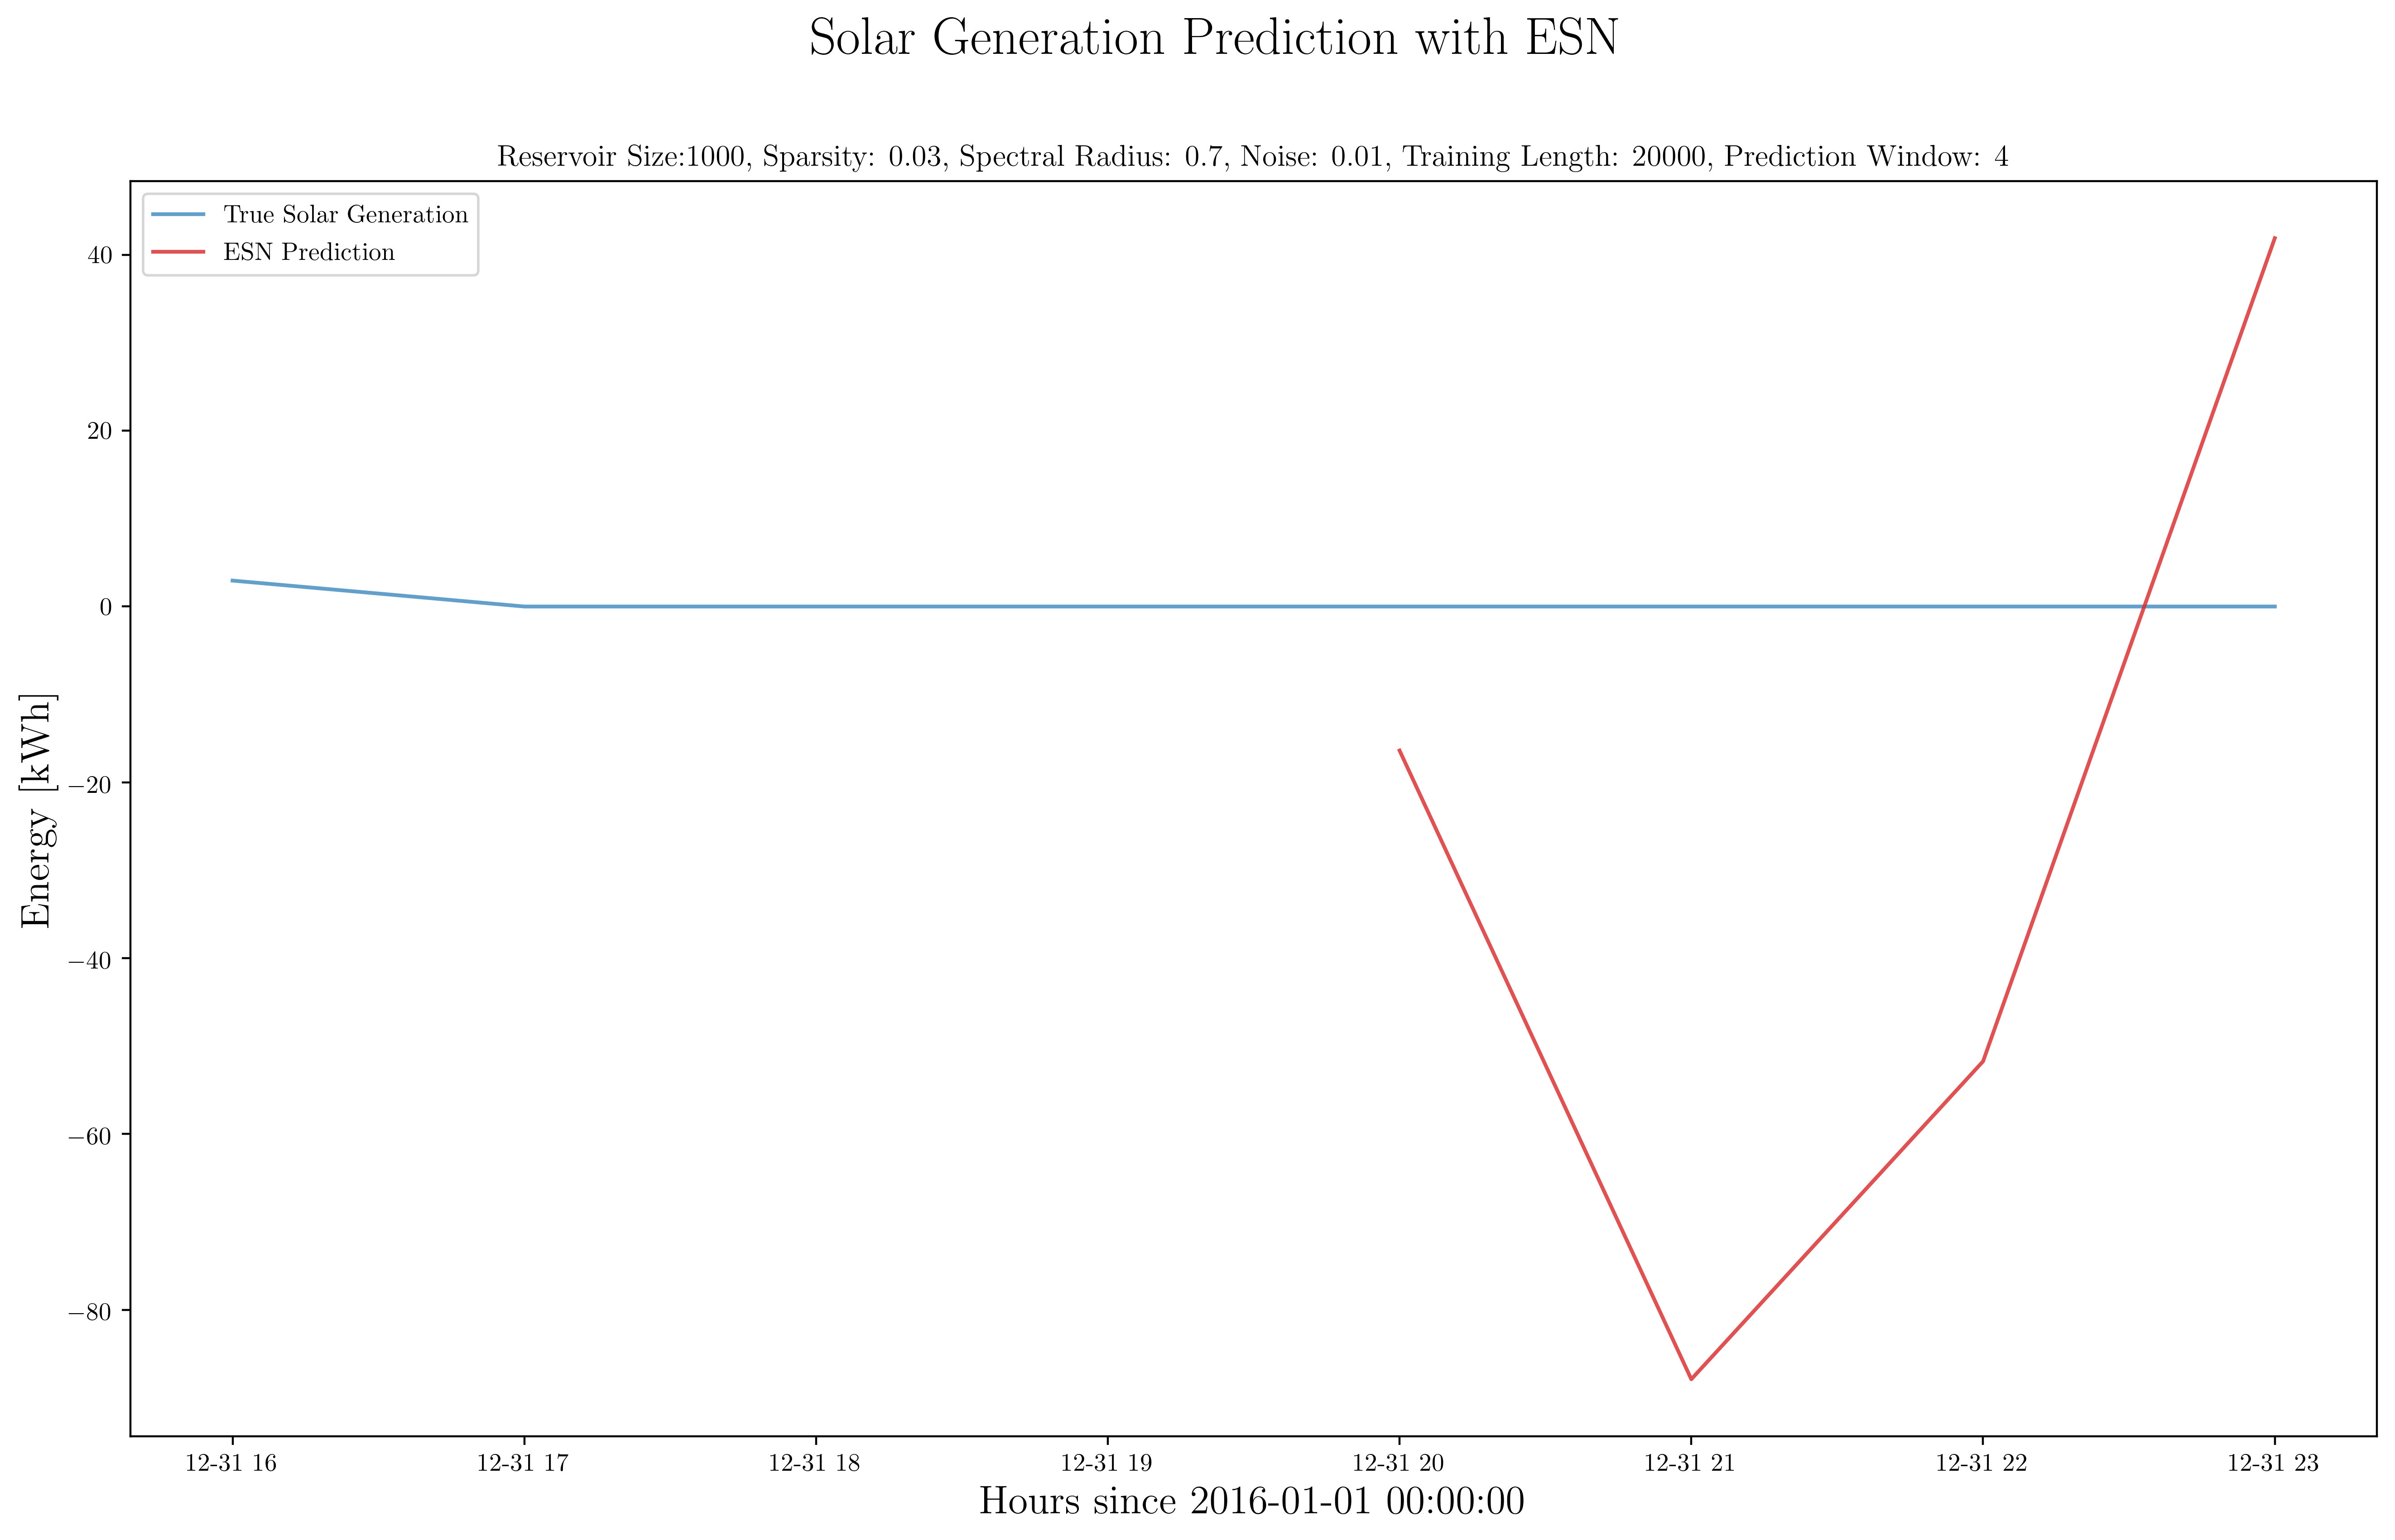
\includegraphics[width=0.8\textwidth]{04_solar_wettemp_prediction.png}
  %% Creator: Matplotlib, PGF backend
%%
%% To include the figure in your LaTeX document, write
%%   \input{<filename>.pgf}
%%
%% Make sure the required packages are loaded in your preamble
%%   \usepackage{pgf}
%%
%% Figures using additional raster images can only be included by \input if
%% they are in the same directory as the main LaTeX file. For loading figures
%% from other directories you can use the `import` package
%%   \usepackage{import}
%% and then include the figures with
%%   \import{<path to file>}{<filename>.pgf}
%%
%% Matplotlib used the following preamble
%%
\begingroup%
\makeatletter%
\begin{pgfpicture}%
\pgfpathrectangle{\pgfpointorigin}{\pgfqpoint{5.531696in}{3.164528in}}%
\pgfusepath{use as bounding box, clip}%
\begin{pgfscope}%
\pgfsetbuttcap%
\pgfsetmiterjoin%
\definecolor{currentfill}{rgb}{1.000000,1.000000,1.000000}%
\pgfsetfillcolor{currentfill}%
\pgfsetlinewidth{0.000000pt}%
\definecolor{currentstroke}{rgb}{1.000000,1.000000,1.000000}%
\pgfsetstrokecolor{currentstroke}%
\pgfsetdash{}{0pt}%
\pgfpathmoveto{\pgfqpoint{0.000000in}{0.000000in}}%
\pgfpathlineto{\pgfqpoint{5.531696in}{0.000000in}}%
\pgfpathlineto{\pgfqpoint{5.531696in}{3.164528in}}%
\pgfpathlineto{\pgfqpoint{0.000000in}{3.164528in}}%
\pgfpathclose%
\pgfusepath{fill}%
\end{pgfscope}%
\begin{pgfscope}%
\pgfsetbuttcap%
\pgfsetmiterjoin%
\definecolor{currentfill}{rgb}{1.000000,1.000000,1.000000}%
\pgfsetfillcolor{currentfill}%
\pgfsetlinewidth{0.000000pt}%
\definecolor{currentstroke}{rgb}{0.000000,0.000000,0.000000}%
\pgfsetstrokecolor{currentstroke}%
\pgfsetstrokeopacity{0.000000}%
\pgfsetdash{}{0pt}%
\pgfpathmoveto{\pgfqpoint{0.669445in}{0.499691in}}%
\pgfpathlineto{\pgfqpoint{5.431696in}{0.499691in}}%
\pgfpathlineto{\pgfqpoint{5.431696in}{2.865455in}}%
\pgfpathlineto{\pgfqpoint{0.669445in}{2.865455in}}%
\pgfpathclose%
\pgfusepath{fill}%
\end{pgfscope}%
\begin{pgfscope}%
\pgfpathrectangle{\pgfqpoint{0.669445in}{0.499691in}}{\pgfqpoint{4.762251in}{2.365763in}}%
\pgfusepath{clip}%
\pgfsetbuttcap%
\pgfsetroundjoin%
\definecolor{currentfill}{rgb}{0.501961,0.501961,0.501961}%
\pgfsetfillcolor{currentfill}%
\pgfsetfillopacity{0.600000}%
\pgfsetlinewidth{1.003750pt}%
\definecolor{currentstroke}{rgb}{0.501961,0.501961,0.501961}%
\pgfsetstrokecolor{currentstroke}%
\pgfsetstrokeopacity{0.600000}%
\pgfsetdash{}{0pt}%
\pgfpathmoveto{\pgfqpoint{3.118928in}{0.961895in}}%
\pgfpathlineto{\pgfqpoint{3.118928in}{0.967206in}}%
\pgfpathlineto{\pgfqpoint{3.164500in}{0.967206in}}%
\pgfpathlineto{\pgfqpoint{3.210072in}{0.967206in}}%
\pgfpathlineto{\pgfqpoint{3.255644in}{0.967206in}}%
\pgfpathlineto{\pgfqpoint{3.301216in}{0.967206in}}%
\pgfpathlineto{\pgfqpoint{3.346787in}{0.967206in}}%
\pgfpathlineto{\pgfqpoint{3.392359in}{0.967206in}}%
\pgfpathlineto{\pgfqpoint{3.392359in}{0.607226in}}%
\pgfpathlineto{\pgfqpoint{3.392359in}{0.607226in}}%
\pgfpathlineto{\pgfqpoint{3.346787in}{0.822671in}}%
\pgfpathlineto{\pgfqpoint{3.301216in}{0.887143in}}%
\pgfpathlineto{\pgfqpoint{3.255644in}{0.927621in}}%
\pgfpathlineto{\pgfqpoint{3.210072in}{0.884507in}}%
\pgfpathlineto{\pgfqpoint{3.164500in}{0.940777in}}%
\pgfpathlineto{\pgfqpoint{3.118928in}{0.961895in}}%
\pgfpathclose%
\pgfusepath{stroke,fill}%
\end{pgfscope}%
\begin{pgfscope}%
\pgfpathrectangle{\pgfqpoint{0.669445in}{0.499691in}}{\pgfqpoint{4.762251in}{2.365763in}}%
\pgfusepath{clip}%
\pgfsetbuttcap%
\pgfsetroundjoin%
\definecolor{currentfill}{rgb}{0.501961,0.501961,0.501961}%
\pgfsetfillcolor{currentfill}%
\pgfsetfillopacity{0.600000}%
\pgfsetlinewidth{1.003750pt}%
\definecolor{currentstroke}{rgb}{0.501961,0.501961,0.501961}%
\pgfsetstrokecolor{currentstroke}%
\pgfsetstrokeopacity{0.600000}%
\pgfsetdash{}{0pt}%
\pgfpathmoveto{\pgfqpoint{3.802505in}{0.893433in}}%
\pgfpathlineto{\pgfqpoint{3.802505in}{0.967206in}}%
\pgfpathlineto{\pgfqpoint{3.848077in}{0.967206in}}%
\pgfpathlineto{\pgfqpoint{3.893649in}{0.967206in}}%
\pgfpathlineto{\pgfqpoint{3.893649in}{0.926687in}}%
\pgfpathlineto{\pgfqpoint{3.893649in}{0.926687in}}%
\pgfpathlineto{\pgfqpoint{3.848077in}{0.819777in}}%
\pgfpathlineto{\pgfqpoint{3.802505in}{0.893433in}}%
\pgfpathclose%
\pgfusepath{stroke,fill}%
\end{pgfscope}%
\begin{pgfscope}%
\pgfpathrectangle{\pgfqpoint{0.669445in}{0.499691in}}{\pgfqpoint{4.762251in}{2.365763in}}%
\pgfusepath{clip}%
\pgfsetbuttcap%
\pgfsetroundjoin%
\definecolor{currentfill}{rgb}{0.501961,0.501961,0.501961}%
\pgfsetfillcolor{currentfill}%
\pgfsetfillopacity{0.600000}%
\pgfsetlinewidth{1.003750pt}%
\definecolor{currentstroke}{rgb}{0.501961,0.501961,0.501961}%
\pgfsetstrokecolor{currentstroke}%
\pgfsetstrokeopacity{0.600000}%
\pgfsetdash{}{0pt}%
\pgfpathmoveto{\pgfqpoint{3.984792in}{0.958793in}}%
\pgfpathlineto{\pgfqpoint{3.984792in}{0.967206in}}%
\pgfpathlineto{\pgfqpoint{4.030364in}{0.967206in}}%
\pgfpathlineto{\pgfqpoint{4.075936in}{0.967206in}}%
\pgfpathlineto{\pgfqpoint{4.121508in}{0.967206in}}%
\pgfpathlineto{\pgfqpoint{4.121508in}{0.699858in}}%
\pgfpathlineto{\pgfqpoint{4.121508in}{0.699858in}}%
\pgfpathlineto{\pgfqpoint{4.075936in}{0.857751in}}%
\pgfpathlineto{\pgfqpoint{4.030364in}{0.960216in}}%
\pgfpathlineto{\pgfqpoint{3.984792in}{0.958793in}}%
\pgfpathclose%
\pgfusepath{stroke,fill}%
\end{pgfscope}%
\begin{pgfscope}%
\pgfpathrectangle{\pgfqpoint{0.669445in}{0.499691in}}{\pgfqpoint{4.762251in}{2.365763in}}%
\pgfusepath{clip}%
\pgfsetbuttcap%
\pgfsetroundjoin%
\definecolor{currentfill}{rgb}{0.501961,0.501961,0.501961}%
\pgfsetfillcolor{currentfill}%
\pgfsetfillopacity{0.600000}%
\pgfsetlinewidth{1.003750pt}%
\definecolor{currentstroke}{rgb}{0.501961,0.501961,0.501961}%
\pgfsetstrokecolor{currentstroke}%
\pgfsetstrokeopacity{0.600000}%
\pgfsetdash{}{0pt}%
\pgfpathmoveto{\pgfqpoint{4.349367in}{0.941298in}}%
\pgfpathlineto{\pgfqpoint{4.349367in}{0.967206in}}%
\pgfpathlineto{\pgfqpoint{4.394938in}{0.967206in}}%
\pgfpathlineto{\pgfqpoint{4.394938in}{0.960216in}}%
\pgfpathlineto{\pgfqpoint{4.394938in}{0.960216in}}%
\pgfpathlineto{\pgfqpoint{4.349367in}{0.941298in}}%
\pgfpathclose%
\pgfusepath{stroke,fill}%
\end{pgfscope}%
\begin{pgfscope}%
\pgfpathrectangle{\pgfqpoint{0.669445in}{0.499691in}}{\pgfqpoint{4.762251in}{2.365763in}}%
\pgfusepath{clip}%
\pgfsetbuttcap%
\pgfsetroundjoin%
\definecolor{currentfill}{rgb}{0.501961,0.501961,0.501961}%
\pgfsetfillcolor{currentfill}%
\pgfsetfillopacity{0.600000}%
\pgfsetlinewidth{1.003750pt}%
\definecolor{currentstroke}{rgb}{0.501961,0.501961,0.501961}%
\pgfsetstrokecolor{currentstroke}%
\pgfsetstrokeopacity{0.600000}%
\pgfsetdash{}{0pt}%
\pgfpathmoveto{\pgfqpoint{4.805084in}{0.960185in}}%
\pgfpathlineto{\pgfqpoint{4.805084in}{0.967206in}}%
\pgfpathlineto{\pgfqpoint{4.850656in}{0.967206in}}%
\pgfpathlineto{\pgfqpoint{4.850656in}{0.842149in}}%
\pgfpathlineto{\pgfqpoint{4.850656in}{0.842149in}}%
\pgfpathlineto{\pgfqpoint{4.805084in}{0.960185in}}%
\pgfpathclose%
\pgfusepath{stroke,fill}%
\end{pgfscope}%
\begin{pgfscope}%
\pgfpathrectangle{\pgfqpoint{0.669445in}{0.499691in}}{\pgfqpoint{4.762251in}{2.365763in}}%
\pgfusepath{clip}%
\pgfsetbuttcap%
\pgfsetroundjoin%
\definecolor{currentfill}{rgb}{0.501961,0.501961,0.501961}%
\pgfsetfillcolor{currentfill}%
\pgfsetfillopacity{0.600000}%
\pgfsetlinewidth{1.003750pt}%
\definecolor{currentstroke}{rgb}{0.501961,0.501961,0.501961}%
\pgfsetstrokecolor{currentstroke}%
\pgfsetstrokeopacity{0.600000}%
\pgfsetdash{}{0pt}%
\pgfpathmoveto{\pgfqpoint{5.078515in}{0.966029in}}%
\pgfpathlineto{\pgfqpoint{5.078515in}{0.967206in}}%
\pgfpathlineto{\pgfqpoint{5.124087in}{0.967206in}}%
\pgfpathlineto{\pgfqpoint{5.169659in}{0.967206in}}%
\pgfpathlineto{\pgfqpoint{5.215230in}{0.967206in}}%
\pgfpathlineto{\pgfqpoint{5.215230in}{0.706218in}}%
\pgfpathlineto{\pgfqpoint{5.215230in}{0.706218in}}%
\pgfpathlineto{\pgfqpoint{5.169659in}{0.865217in}}%
\pgfpathlineto{\pgfqpoint{5.124087in}{0.940906in}}%
\pgfpathlineto{\pgfqpoint{5.078515in}{0.966029in}}%
\pgfpathclose%
\pgfusepath{stroke,fill}%
\end{pgfscope}%
\begin{pgfscope}%
\pgfsetbuttcap%
\pgfsetroundjoin%
\definecolor{currentfill}{rgb}{0.000000,0.000000,0.000000}%
\pgfsetfillcolor{currentfill}%
\pgfsetlinewidth{0.803000pt}%
\definecolor{currentstroke}{rgb}{0.000000,0.000000,0.000000}%
\pgfsetstrokecolor{currentstroke}%
\pgfsetdash{}{0pt}%
\pgfsys@defobject{currentmarker}{\pgfqpoint{0.000000in}{-0.048611in}}{\pgfqpoint{0.000000in}{0.000000in}}{%
\pgfpathmoveto{\pgfqpoint{0.000000in}{0.000000in}}%
\pgfpathlineto{\pgfqpoint{0.000000in}{-0.048611in}}%
\pgfusepath{stroke,fill}%
}%
\begin{pgfscope}%
\pgfsys@transformshift{1.432773in}{0.499691in}%
\pgfsys@useobject{currentmarker}{}%
\end{pgfscope}%
\end{pgfscope}%
\begin{pgfscope}%
\definecolor{textcolor}{rgb}{0.000000,0.000000,0.000000}%
\pgfsetstrokecolor{textcolor}%
\pgfsetfillcolor{textcolor}%
\pgftext[x=1.432773in,y=0.402469in,,top]{\color{textcolor}\rmfamily\fontsize{10.000000}{12.000000}\selectfont \(\displaystyle 26220\)}%
\end{pgfscope}%
\begin{pgfscope}%
\pgfsetbuttcap%
\pgfsetroundjoin%
\definecolor{currentfill}{rgb}{0.000000,0.000000,0.000000}%
\pgfsetfillcolor{currentfill}%
\pgfsetlinewidth{0.803000pt}%
\definecolor{currentstroke}{rgb}{0.000000,0.000000,0.000000}%
\pgfsetstrokecolor{currentstroke}%
\pgfsetdash{}{0pt}%
\pgfsys@defobject{currentmarker}{\pgfqpoint{0.000000in}{-0.048611in}}{\pgfqpoint{0.000000in}{0.000000in}}{%
\pgfpathmoveto{\pgfqpoint{0.000000in}{0.000000in}}%
\pgfpathlineto{\pgfqpoint{0.000000in}{-0.048611in}}%
\pgfusepath{stroke,fill}%
}%
\begin{pgfscope}%
\pgfsys@transformshift{2.344208in}{0.499691in}%
\pgfsys@useobject{currentmarker}{}%
\end{pgfscope}%
\end{pgfscope}%
\begin{pgfscope}%
\definecolor{textcolor}{rgb}{0.000000,0.000000,0.000000}%
\pgfsetstrokecolor{textcolor}%
\pgfsetfillcolor{textcolor}%
\pgftext[x=2.344208in,y=0.402469in,,top]{\color{textcolor}\rmfamily\fontsize{10.000000}{12.000000}\selectfont \(\displaystyle 26240\)}%
\end{pgfscope}%
\begin{pgfscope}%
\pgfsetbuttcap%
\pgfsetroundjoin%
\definecolor{currentfill}{rgb}{0.000000,0.000000,0.000000}%
\pgfsetfillcolor{currentfill}%
\pgfsetlinewidth{0.803000pt}%
\definecolor{currentstroke}{rgb}{0.000000,0.000000,0.000000}%
\pgfsetstrokecolor{currentstroke}%
\pgfsetdash{}{0pt}%
\pgfsys@defobject{currentmarker}{\pgfqpoint{0.000000in}{-0.048611in}}{\pgfqpoint{0.000000in}{0.000000in}}{%
\pgfpathmoveto{\pgfqpoint{0.000000in}{0.000000in}}%
\pgfpathlineto{\pgfqpoint{0.000000in}{-0.048611in}}%
\pgfusepath{stroke,fill}%
}%
\begin{pgfscope}%
\pgfsys@transformshift{3.255644in}{0.499691in}%
\pgfsys@useobject{currentmarker}{}%
\end{pgfscope}%
\end{pgfscope}%
\begin{pgfscope}%
\definecolor{textcolor}{rgb}{0.000000,0.000000,0.000000}%
\pgfsetstrokecolor{textcolor}%
\pgfsetfillcolor{textcolor}%
\pgftext[x=3.255644in,y=0.402469in,,top]{\color{textcolor}\rmfamily\fontsize{10.000000}{12.000000}\selectfont \(\displaystyle 26260\)}%
\end{pgfscope}%
\begin{pgfscope}%
\pgfsetbuttcap%
\pgfsetroundjoin%
\definecolor{currentfill}{rgb}{0.000000,0.000000,0.000000}%
\pgfsetfillcolor{currentfill}%
\pgfsetlinewidth{0.803000pt}%
\definecolor{currentstroke}{rgb}{0.000000,0.000000,0.000000}%
\pgfsetstrokecolor{currentstroke}%
\pgfsetdash{}{0pt}%
\pgfsys@defobject{currentmarker}{\pgfqpoint{0.000000in}{-0.048611in}}{\pgfqpoint{0.000000in}{0.000000in}}{%
\pgfpathmoveto{\pgfqpoint{0.000000in}{0.000000in}}%
\pgfpathlineto{\pgfqpoint{0.000000in}{-0.048611in}}%
\pgfusepath{stroke,fill}%
}%
\begin{pgfscope}%
\pgfsys@transformshift{4.167079in}{0.499691in}%
\pgfsys@useobject{currentmarker}{}%
\end{pgfscope}%
\end{pgfscope}%
\begin{pgfscope}%
\definecolor{textcolor}{rgb}{0.000000,0.000000,0.000000}%
\pgfsetstrokecolor{textcolor}%
\pgfsetfillcolor{textcolor}%
\pgftext[x=4.167079in,y=0.402469in,,top]{\color{textcolor}\rmfamily\fontsize{10.000000}{12.000000}\selectfont \(\displaystyle 26280\)}%
\end{pgfscope}%
\begin{pgfscope}%
\pgfsetbuttcap%
\pgfsetroundjoin%
\definecolor{currentfill}{rgb}{0.000000,0.000000,0.000000}%
\pgfsetfillcolor{currentfill}%
\pgfsetlinewidth{0.803000pt}%
\definecolor{currentstroke}{rgb}{0.000000,0.000000,0.000000}%
\pgfsetstrokecolor{currentstroke}%
\pgfsetdash{}{0pt}%
\pgfsys@defobject{currentmarker}{\pgfqpoint{0.000000in}{-0.048611in}}{\pgfqpoint{0.000000in}{0.000000in}}{%
\pgfpathmoveto{\pgfqpoint{0.000000in}{0.000000in}}%
\pgfpathlineto{\pgfqpoint{0.000000in}{-0.048611in}}%
\pgfusepath{stroke,fill}%
}%
\begin{pgfscope}%
\pgfsys@transformshift{5.078515in}{0.499691in}%
\pgfsys@useobject{currentmarker}{}%
\end{pgfscope}%
\end{pgfscope}%
\begin{pgfscope}%
\definecolor{textcolor}{rgb}{0.000000,0.000000,0.000000}%
\pgfsetstrokecolor{textcolor}%
\pgfsetfillcolor{textcolor}%
\pgftext[x=5.078515in,y=0.402469in,,top]{\color{textcolor}\rmfamily\fontsize{10.000000}{12.000000}\selectfont \(\displaystyle 26300\)}%
\end{pgfscope}%
\begin{pgfscope}%
\definecolor{textcolor}{rgb}{0.000000,0.000000,0.000000}%
\pgfsetstrokecolor{textcolor}%
\pgfsetfillcolor{textcolor}%
\pgftext[x=3.050571in,y=0.223457in,,top]{\color{textcolor}\rmfamily\fontsize{10.000000}{12.000000}\selectfont Hours since 2016-01-01 00:00:00}%
\end{pgfscope}%
\begin{pgfscope}%
\pgfsetbuttcap%
\pgfsetroundjoin%
\definecolor{currentfill}{rgb}{0.000000,0.000000,0.000000}%
\pgfsetfillcolor{currentfill}%
\pgfsetlinewidth{0.803000pt}%
\definecolor{currentstroke}{rgb}{0.000000,0.000000,0.000000}%
\pgfsetstrokecolor{currentstroke}%
\pgfsetdash{}{0pt}%
\pgfsys@defobject{currentmarker}{\pgfqpoint{-0.048611in}{0.000000in}}{\pgfqpoint{0.000000in}{0.000000in}}{%
\pgfpathmoveto{\pgfqpoint{0.000000in}{0.000000in}}%
\pgfpathlineto{\pgfqpoint{-0.048611in}{0.000000in}}%
\pgfusepath{stroke,fill}%
}%
\begin{pgfscope}%
\pgfsys@transformshift{0.669445in}{0.967206in}%
\pgfsys@useobject{currentmarker}{}%
\end{pgfscope}%
\end{pgfscope}%
\begin{pgfscope}%
\definecolor{textcolor}{rgb}{0.000000,0.000000,0.000000}%
\pgfsetstrokecolor{textcolor}%
\pgfsetfillcolor{textcolor}%
\pgftext[x=0.502778in,y=0.918980in,left,base]{\color{textcolor}\rmfamily\fontsize{10.000000}{12.000000}\selectfont \(\displaystyle 0\)}%
\end{pgfscope}%
\begin{pgfscope}%
\pgfsetbuttcap%
\pgfsetroundjoin%
\definecolor{currentfill}{rgb}{0.000000,0.000000,0.000000}%
\pgfsetfillcolor{currentfill}%
\pgfsetlinewidth{0.803000pt}%
\definecolor{currentstroke}{rgb}{0.000000,0.000000,0.000000}%
\pgfsetstrokecolor{currentstroke}%
\pgfsetdash{}{0pt}%
\pgfsys@defobject{currentmarker}{\pgfqpoint{-0.048611in}{0.000000in}}{\pgfqpoint{0.000000in}{0.000000in}}{%
\pgfpathmoveto{\pgfqpoint{0.000000in}{0.000000in}}%
\pgfpathlineto{\pgfqpoint{-0.048611in}{0.000000in}}%
\pgfusepath{stroke,fill}%
}%
\begin{pgfscope}%
\pgfsys@transformshift{0.669445in}{1.513822in}%
\pgfsys@useobject{currentmarker}{}%
\end{pgfscope}%
\end{pgfscope}%
\begin{pgfscope}%
\definecolor{textcolor}{rgb}{0.000000,0.000000,0.000000}%
\pgfsetstrokecolor{textcolor}%
\pgfsetfillcolor{textcolor}%
\pgftext[x=0.294444in,y=1.465596in,left,base]{\color{textcolor}\rmfamily\fontsize{10.000000}{12.000000}\selectfont \(\displaystyle 1000\)}%
\end{pgfscope}%
\begin{pgfscope}%
\pgfsetbuttcap%
\pgfsetroundjoin%
\definecolor{currentfill}{rgb}{0.000000,0.000000,0.000000}%
\pgfsetfillcolor{currentfill}%
\pgfsetlinewidth{0.803000pt}%
\definecolor{currentstroke}{rgb}{0.000000,0.000000,0.000000}%
\pgfsetstrokecolor{currentstroke}%
\pgfsetdash{}{0pt}%
\pgfsys@defobject{currentmarker}{\pgfqpoint{-0.048611in}{0.000000in}}{\pgfqpoint{0.000000in}{0.000000in}}{%
\pgfpathmoveto{\pgfqpoint{0.000000in}{0.000000in}}%
\pgfpathlineto{\pgfqpoint{-0.048611in}{0.000000in}}%
\pgfusepath{stroke,fill}%
}%
\begin{pgfscope}%
\pgfsys@transformshift{0.669445in}{2.060438in}%
\pgfsys@useobject{currentmarker}{}%
\end{pgfscope}%
\end{pgfscope}%
\begin{pgfscope}%
\definecolor{textcolor}{rgb}{0.000000,0.000000,0.000000}%
\pgfsetstrokecolor{textcolor}%
\pgfsetfillcolor{textcolor}%
\pgftext[x=0.294444in,y=2.012212in,left,base]{\color{textcolor}\rmfamily\fontsize{10.000000}{12.000000}\selectfont \(\displaystyle 2000\)}%
\end{pgfscope}%
\begin{pgfscope}%
\pgfsetbuttcap%
\pgfsetroundjoin%
\definecolor{currentfill}{rgb}{0.000000,0.000000,0.000000}%
\pgfsetfillcolor{currentfill}%
\pgfsetlinewidth{0.803000pt}%
\definecolor{currentstroke}{rgb}{0.000000,0.000000,0.000000}%
\pgfsetstrokecolor{currentstroke}%
\pgfsetdash{}{0pt}%
\pgfsys@defobject{currentmarker}{\pgfqpoint{-0.048611in}{0.000000in}}{\pgfqpoint{0.000000in}{0.000000in}}{%
\pgfpathmoveto{\pgfqpoint{0.000000in}{0.000000in}}%
\pgfpathlineto{\pgfqpoint{-0.048611in}{0.000000in}}%
\pgfusepath{stroke,fill}%
}%
\begin{pgfscope}%
\pgfsys@transformshift{0.669445in}{2.607054in}%
\pgfsys@useobject{currentmarker}{}%
\end{pgfscope}%
\end{pgfscope}%
\begin{pgfscope}%
\definecolor{textcolor}{rgb}{0.000000,0.000000,0.000000}%
\pgfsetstrokecolor{textcolor}%
\pgfsetfillcolor{textcolor}%
\pgftext[x=0.294444in,y=2.558829in,left,base]{\color{textcolor}\rmfamily\fontsize{10.000000}{12.000000}\selectfont \(\displaystyle 3000\)}%
\end{pgfscope}%
\begin{pgfscope}%
\definecolor{textcolor}{rgb}{0.000000,0.000000,0.000000}%
\pgfsetstrokecolor{textcolor}%
\pgfsetfillcolor{textcolor}%
\pgftext[x=0.238889in,y=1.682573in,,bottom,rotate=90.000000]{\color{textcolor}\rmfamily\fontsize{10.000000}{12.000000}\selectfont Energy [kWh]}%
\end{pgfscope}%
\begin{pgfscope}%
\pgfpathrectangle{\pgfqpoint{0.669445in}{0.499691in}}{\pgfqpoint{4.762251in}{2.365763in}}%
\pgfusepath{clip}%
\pgfsetrectcap%
\pgfsetroundjoin%
\pgfsetlinewidth{1.505625pt}%
\definecolor{currentstroke}{rgb}{0.121569,0.466667,0.705882}%
\pgfsetstrokecolor{currentstroke}%
\pgfsetstrokeopacity{0.700000}%
\pgfsetdash{}{0pt}%
\pgfpathmoveto{\pgfqpoint{0.885911in}{0.967206in}}%
\pgfpathlineto{\pgfqpoint{0.931483in}{0.967206in}}%
\pgfpathlineto{\pgfqpoint{0.977055in}{0.967206in}}%
\pgfpathlineto{\pgfqpoint{1.022627in}{0.967206in}}%
\pgfpathlineto{\pgfqpoint{1.068198in}{0.967206in}}%
\pgfpathlineto{\pgfqpoint{1.113770in}{0.967206in}}%
\pgfpathlineto{\pgfqpoint{1.159342in}{0.967206in}}%
\pgfpathlineto{\pgfqpoint{1.204914in}{0.972342in}}%
\pgfpathlineto{\pgfqpoint{1.250485in}{1.090331in}}%
\pgfpathlineto{\pgfqpoint{1.296057in}{1.116705in}}%
\pgfpathlineto{\pgfqpoint{1.341629in}{1.161528in}}%
\pgfpathlineto{\pgfqpoint{1.387201in}{1.158248in}}%
\pgfpathlineto{\pgfqpoint{1.432773in}{1.151962in}}%
\pgfpathlineto{\pgfqpoint{1.478344in}{1.128184in}}%
\pgfpathlineto{\pgfqpoint{1.523916in}{1.088691in}}%
\pgfpathlineto{\pgfqpoint{1.569488in}{1.019599in}}%
\pgfpathlineto{\pgfqpoint{1.615060in}{0.971084in}}%
\pgfpathlineto{\pgfqpoint{1.660631in}{0.967206in}}%
\pgfpathlineto{\pgfqpoint{1.706203in}{0.967206in}}%
\pgfpathlineto{\pgfqpoint{1.751775in}{0.967206in}}%
\pgfpathlineto{\pgfqpoint{1.797347in}{0.967206in}}%
\pgfpathlineto{\pgfqpoint{1.842919in}{0.967206in}}%
\pgfpathlineto{\pgfqpoint{1.888490in}{0.967206in}}%
\pgfpathlineto{\pgfqpoint{1.934062in}{0.967206in}}%
\pgfpathlineto{\pgfqpoint{1.979634in}{0.967206in}}%
\pgfpathlineto{\pgfqpoint{2.025206in}{0.967206in}}%
\pgfpathlineto{\pgfqpoint{2.070778in}{0.967206in}}%
\pgfpathlineto{\pgfqpoint{2.116349in}{0.967206in}}%
\pgfpathlineto{\pgfqpoint{2.161921in}{0.967206in}}%
\pgfpathlineto{\pgfqpoint{2.207493in}{0.967206in}}%
\pgfpathlineto{\pgfqpoint{2.253065in}{0.967206in}}%
\pgfpathlineto{\pgfqpoint{2.298636in}{1.009056in}}%
\pgfpathlineto{\pgfqpoint{2.344208in}{1.305014in}}%
\pgfpathlineto{\pgfqpoint{2.389780in}{1.790819in}}%
\pgfpathlineto{\pgfqpoint{2.435352in}{1.525574in}}%
\pgfpathlineto{\pgfqpoint{2.480924in}{1.569303in}}%
\pgfpathlineto{\pgfqpoint{2.526495in}{1.447408in}}%
\pgfpathlineto{\pgfqpoint{2.572067in}{1.377851in}}%
\pgfpathlineto{\pgfqpoint{2.617639in}{1.162894in}}%
\pgfpathlineto{\pgfqpoint{2.663211in}{1.041791in}}%
\pgfpathlineto{\pgfqpoint{2.708782in}{0.970767in}}%
\pgfpathlineto{\pgfqpoint{2.754354in}{0.967206in}}%
\pgfpathlineto{\pgfqpoint{2.799926in}{0.967206in}}%
\pgfpathlineto{\pgfqpoint{2.845498in}{0.967206in}}%
\pgfpathlineto{\pgfqpoint{2.891070in}{0.967206in}}%
\pgfpathlineto{\pgfqpoint{2.936641in}{0.967206in}}%
\pgfpathlineto{\pgfqpoint{2.982213in}{0.967206in}}%
\pgfpathlineto{\pgfqpoint{3.027785in}{0.967206in}}%
\pgfpathlineto{\pgfqpoint{3.073357in}{0.967206in}}%
\pgfpathlineto{\pgfqpoint{3.118928in}{0.967206in}}%
\pgfpathlineto{\pgfqpoint{3.164500in}{0.967206in}}%
\pgfpathlineto{\pgfqpoint{3.210072in}{0.967206in}}%
\pgfpathlineto{\pgfqpoint{3.255644in}{0.967206in}}%
\pgfpathlineto{\pgfqpoint{3.301216in}{0.967206in}}%
\pgfpathlineto{\pgfqpoint{3.346787in}{0.967206in}}%
\pgfpathlineto{\pgfqpoint{3.392359in}{1.022702in}}%
\pgfpathlineto{\pgfqpoint{3.437931in}{1.264155in}}%
\pgfpathlineto{\pgfqpoint{3.483503in}{1.558508in}}%
\pgfpathlineto{\pgfqpoint{3.529074in}{2.547473in}}%
\pgfpathlineto{\pgfqpoint{3.574646in}{2.757920in}}%
\pgfpathlineto{\pgfqpoint{3.620218in}{2.474089in}}%
\pgfpathlineto{\pgfqpoint{3.665790in}{1.976122in}}%
\pgfpathlineto{\pgfqpoint{3.711362in}{1.490317in}}%
\pgfpathlineto{\pgfqpoint{3.756933in}{1.202114in}}%
\pgfpathlineto{\pgfqpoint{3.802505in}{0.985487in}}%
\pgfpathlineto{\pgfqpoint{3.848077in}{0.967206in}}%
\pgfpathlineto{\pgfqpoint{3.893649in}{0.967206in}}%
\pgfpathlineto{\pgfqpoint{3.939220in}{0.967206in}}%
\pgfpathlineto{\pgfqpoint{3.984792in}{0.967206in}}%
\pgfpathlineto{\pgfqpoint{4.030364in}{0.967206in}}%
\pgfpathlineto{\pgfqpoint{4.075936in}{0.967206in}}%
\pgfpathlineto{\pgfqpoint{4.121508in}{0.967206in}}%
\pgfpathlineto{\pgfqpoint{4.167079in}{0.967206in}}%
\pgfpathlineto{\pgfqpoint{4.212651in}{0.967206in}}%
\pgfpathlineto{\pgfqpoint{4.258223in}{0.967206in}}%
\pgfpathlineto{\pgfqpoint{4.303795in}{0.967206in}}%
\pgfpathlineto{\pgfqpoint{4.349367in}{0.967206in}}%
\pgfpathlineto{\pgfqpoint{4.394938in}{0.967206in}}%
\pgfpathlineto{\pgfqpoint{4.440510in}{0.967206in}}%
\pgfpathlineto{\pgfqpoint{4.486082in}{0.967955in}}%
\pgfpathlineto{\pgfqpoint{4.531654in}{0.976508in}}%
\pgfpathlineto{\pgfqpoint{4.577225in}{0.992801in}}%
\pgfpathlineto{\pgfqpoint{4.622797in}{1.022318in}}%
\pgfpathlineto{\pgfqpoint{4.668369in}{1.018041in}}%
\pgfpathlineto{\pgfqpoint{4.713941in}{1.109599in}}%
\pgfpathlineto{\pgfqpoint{4.759513in}{1.136520in}}%
\pgfpathlineto{\pgfqpoint{4.805084in}{1.075299in}}%
\pgfpathlineto{\pgfqpoint{4.850656in}{1.006740in}}%
\pgfpathlineto{\pgfqpoint{4.896228in}{0.968817in}}%
\pgfpathlineto{\pgfqpoint{4.941800in}{0.967206in}}%
\pgfpathlineto{\pgfqpoint{4.987371in}{0.967206in}}%
\pgfpathlineto{\pgfqpoint{5.032943in}{0.967206in}}%
\pgfpathlineto{\pgfqpoint{5.078515in}{0.967206in}}%
\pgfpathlineto{\pgfqpoint{5.124087in}{0.967206in}}%
\pgfpathlineto{\pgfqpoint{5.169659in}{0.967206in}}%
\pgfpathlineto{\pgfqpoint{5.215230in}{0.967206in}}%
\pgfusepath{stroke}%
\end{pgfscope}%
\begin{pgfscope}%
\pgfpathrectangle{\pgfqpoint{0.669445in}{0.499691in}}{\pgfqpoint{4.762251in}{2.365763in}}%
\pgfusepath{clip}%
\pgfsetrectcap%
\pgfsetroundjoin%
\pgfsetlinewidth{1.505625pt}%
\definecolor{currentstroke}{rgb}{0.839216,0.152941,0.156863}%
\pgfsetstrokecolor{currentstroke}%
\pgfsetstrokeopacity{0.800000}%
\pgfsetdash{}{0pt}%
\pgfpathmoveto{\pgfqpoint{3.073357in}{0.975883in}}%
\pgfpathlineto{\pgfqpoint{3.118928in}{0.961895in}}%
\pgfpathlineto{\pgfqpoint{3.164500in}{0.940777in}}%
\pgfpathlineto{\pgfqpoint{3.210072in}{0.884507in}}%
\pgfpathlineto{\pgfqpoint{3.255644in}{0.927621in}}%
\pgfpathlineto{\pgfqpoint{3.301216in}{0.887143in}}%
\pgfpathlineto{\pgfqpoint{3.346787in}{0.822671in}}%
\pgfpathlineto{\pgfqpoint{3.392359in}{0.607226in}}%
\pgfpathlineto{\pgfqpoint{3.437931in}{1.292155in}}%
\pgfpathlineto{\pgfqpoint{3.483503in}{1.781032in}}%
\pgfpathlineto{\pgfqpoint{3.529074in}{2.231018in}}%
\pgfpathlineto{\pgfqpoint{3.574646in}{2.490747in}}%
\pgfpathlineto{\pgfqpoint{3.620218in}{2.717582in}}%
\pgfpathlineto{\pgfqpoint{3.665790in}{2.305087in}}%
\pgfpathlineto{\pgfqpoint{3.711362in}{1.795419in}}%
\pgfpathlineto{\pgfqpoint{3.756933in}{1.152327in}}%
\pgfpathlineto{\pgfqpoint{3.802505in}{0.893433in}}%
\pgfpathlineto{\pgfqpoint{3.848077in}{0.819777in}}%
\pgfpathlineto{\pgfqpoint{3.893649in}{0.926687in}}%
\pgfpathlineto{\pgfqpoint{3.939220in}{1.171968in}}%
\pgfpathlineto{\pgfqpoint{3.984792in}{0.958793in}}%
\pgfpathlineto{\pgfqpoint{4.030364in}{0.960216in}}%
\pgfpathlineto{\pgfqpoint{4.075936in}{0.857751in}}%
\pgfpathlineto{\pgfqpoint{4.121508in}{0.699858in}}%
\pgfpathlineto{\pgfqpoint{4.167079in}{1.008927in}}%
\pgfpathlineto{\pgfqpoint{4.212651in}{1.089518in}}%
\pgfpathlineto{\pgfqpoint{4.258223in}{1.219709in}}%
\pgfpathlineto{\pgfqpoint{4.303795in}{1.342772in}}%
\pgfpathlineto{\pgfqpoint{4.349367in}{0.941298in}}%
\pgfpathlineto{\pgfqpoint{4.394938in}{0.960216in}}%
\pgfpathlineto{\pgfqpoint{4.440510in}{1.040890in}}%
\pgfpathlineto{\pgfqpoint{4.486082in}{1.179036in}}%
\pgfpathlineto{\pgfqpoint{4.531654in}{1.008202in}}%
\pgfpathlineto{\pgfqpoint{4.577225in}{1.064252in}}%
\pgfpathlineto{\pgfqpoint{4.622797in}{1.164145in}}%
\pgfpathlineto{\pgfqpoint{4.668369in}{1.223399in}}%
\pgfpathlineto{\pgfqpoint{4.713941in}{1.036433in}}%
\pgfpathlineto{\pgfqpoint{4.759513in}{1.035360in}}%
\pgfpathlineto{\pgfqpoint{4.805084in}{0.960185in}}%
\pgfpathlineto{\pgfqpoint{4.850656in}{0.842149in}}%
\pgfpathlineto{\pgfqpoint{4.896228in}{1.082054in}}%
\pgfpathlineto{\pgfqpoint{4.941800in}{1.184194in}}%
\pgfpathlineto{\pgfqpoint{4.987371in}{1.194221in}}%
\pgfpathlineto{\pgfqpoint{5.032943in}{1.092432in}}%
\pgfpathlineto{\pgfqpoint{5.078515in}{0.966029in}}%
\pgfpathlineto{\pgfqpoint{5.124087in}{0.940906in}}%
\pgfpathlineto{\pgfqpoint{5.169659in}{0.865217in}}%
\pgfpathlineto{\pgfqpoint{5.215230in}{0.706218in}}%
\pgfusepath{stroke}%
\end{pgfscope}%
\begin{pgfscope}%
\pgfpathrectangle{\pgfqpoint{0.669445in}{0.499691in}}{\pgfqpoint{4.762251in}{2.365763in}}%
\pgfusepath{clip}%
\pgfsetrectcap%
\pgfsetroundjoin%
\pgfsetlinewidth{1.505625pt}%
\definecolor{currentstroke}{rgb}{0.121569,0.466667,0.705882}%
\pgfsetstrokecolor{currentstroke}%
\pgfsetdash{}{0pt}%
\pgfpathmoveto{\pgfqpoint{0.669445in}{0.967206in}}%
\pgfpathlineto{\pgfqpoint{5.431696in}{0.967206in}}%
\pgfusepath{stroke}%
\end{pgfscope}%
\begin{pgfscope}%
\pgfsetrectcap%
\pgfsetmiterjoin%
\pgfsetlinewidth{0.803000pt}%
\definecolor{currentstroke}{rgb}{0.000000,0.000000,0.000000}%
\pgfsetstrokecolor{currentstroke}%
\pgfsetdash{}{0pt}%
\pgfpathmoveto{\pgfqpoint{0.669445in}{0.499691in}}%
\pgfpathlineto{\pgfqpoint{0.669445in}{2.865455in}}%
\pgfusepath{stroke}%
\end{pgfscope}%
\begin{pgfscope}%
\pgfsetrectcap%
\pgfsetmiterjoin%
\pgfsetlinewidth{0.803000pt}%
\definecolor{currentstroke}{rgb}{0.000000,0.000000,0.000000}%
\pgfsetstrokecolor{currentstroke}%
\pgfsetdash{}{0pt}%
\pgfpathmoveto{\pgfqpoint{5.431696in}{0.499691in}}%
\pgfpathlineto{\pgfqpoint{5.431696in}{2.865455in}}%
\pgfusepath{stroke}%
\end{pgfscope}%
\begin{pgfscope}%
\pgfsetrectcap%
\pgfsetmiterjoin%
\pgfsetlinewidth{0.803000pt}%
\definecolor{currentstroke}{rgb}{0.000000,0.000000,0.000000}%
\pgfsetstrokecolor{currentstroke}%
\pgfsetdash{}{0pt}%
\pgfpathmoveto{\pgfqpoint{0.669445in}{0.499691in}}%
\pgfpathlineto{\pgfqpoint{5.431696in}{0.499691in}}%
\pgfusepath{stroke}%
\end{pgfscope}%
\begin{pgfscope}%
\pgfsetrectcap%
\pgfsetmiterjoin%
\pgfsetlinewidth{0.803000pt}%
\definecolor{currentstroke}{rgb}{0.000000,0.000000,0.000000}%
\pgfsetstrokecolor{currentstroke}%
\pgfsetdash{}{0pt}%
\pgfpathmoveto{\pgfqpoint{0.669445in}{2.865455in}}%
\pgfpathlineto{\pgfqpoint{5.431696in}{2.865455in}}%
\pgfusepath{stroke}%
\end{pgfscope}%
\begin{pgfscope}%
\definecolor{textcolor}{rgb}{0.000000,0.000000,0.000000}%
\pgfsetstrokecolor{textcolor}%
\pgfsetfillcolor{textcolor}%
\pgftext[x=3.050571in,y=2.948788in,,base]{\color{textcolor}\rmfamily\fontsize{12.000000}{14.400000}\selectfont Solar Generation Prediction with an ESN}%
\end{pgfscope}%
\begin{pgfscope}%
\pgfsetbuttcap%
\pgfsetmiterjoin%
\definecolor{currentfill}{rgb}{1.000000,1.000000,1.000000}%
\pgfsetfillcolor{currentfill}%
\pgfsetfillopacity{0.800000}%
\pgfsetlinewidth{1.003750pt}%
\definecolor{currentstroke}{rgb}{0.800000,0.800000,0.800000}%
\pgfsetstrokecolor{currentstroke}%
\pgfsetstrokeopacity{0.800000}%
\pgfsetdash{}{0pt}%
\pgfpathmoveto{\pgfqpoint{0.766667in}{2.366998in}}%
\pgfpathlineto{\pgfqpoint{2.567403in}{2.366998in}}%
\pgfpathquadraticcurveto{\pgfqpoint{2.595181in}{2.366998in}}{\pgfqpoint{2.595181in}{2.394776in}}%
\pgfpathlineto{\pgfqpoint{2.595181in}{2.768232in}}%
\pgfpathquadraticcurveto{\pgfqpoint{2.595181in}{2.796010in}}{\pgfqpoint{2.567403in}{2.796010in}}%
\pgfpathlineto{\pgfqpoint{0.766667in}{2.796010in}}%
\pgfpathquadraticcurveto{\pgfqpoint{0.738890in}{2.796010in}}{\pgfqpoint{0.738890in}{2.768232in}}%
\pgfpathlineto{\pgfqpoint{0.738890in}{2.394776in}}%
\pgfpathquadraticcurveto{\pgfqpoint{0.738890in}{2.366998in}}{\pgfqpoint{0.766667in}{2.366998in}}%
\pgfpathclose%
\pgfusepath{stroke,fill}%
\end{pgfscope}%
\begin{pgfscope}%
\pgfsetrectcap%
\pgfsetroundjoin%
\pgfsetlinewidth{1.505625pt}%
\definecolor{currentstroke}{rgb}{0.121569,0.466667,0.705882}%
\pgfsetstrokecolor{currentstroke}%
\pgfsetstrokeopacity{0.700000}%
\pgfsetdash{}{0pt}%
\pgfpathmoveto{\pgfqpoint{0.794445in}{2.691843in}}%
\pgfpathlineto{\pgfqpoint{1.072223in}{2.691843in}}%
\pgfusepath{stroke}%
\end{pgfscope}%
\begin{pgfscope}%
\definecolor{textcolor}{rgb}{0.000000,0.000000,0.000000}%
\pgfsetstrokecolor{textcolor}%
\pgfsetfillcolor{textcolor}%
\pgftext[x=1.183334in,y=2.643232in,left,base]{\color{textcolor}\rmfamily\fontsize{10.000000}{12.000000}\selectfont True Solar Generation}%
\end{pgfscope}%
\begin{pgfscope}%
\pgfsetrectcap%
\pgfsetroundjoin%
\pgfsetlinewidth{1.505625pt}%
\definecolor{currentstroke}{rgb}{0.839216,0.152941,0.156863}%
\pgfsetstrokecolor{currentstroke}%
\pgfsetstrokeopacity{0.800000}%
\pgfsetdash{}{0pt}%
\pgfpathmoveto{\pgfqpoint{0.794445in}{2.498171in}}%
\pgfpathlineto{\pgfqpoint{1.072223in}{2.498171in}}%
\pgfusepath{stroke}%
\end{pgfscope}%
\begin{pgfscope}%
\definecolor{textcolor}{rgb}{0.000000,0.000000,0.000000}%
\pgfsetstrokecolor{textcolor}%
\pgfsetfillcolor{textcolor}%
\pgftext[x=1.183334in,y=2.449560in,left,base]{\color{textcolor}\rmfamily\fontsize{10.000000}{12.000000}\selectfont ESN Prediction}%
\end{pgfscope}%
\end{pgfpicture}%
\makeatother%
\endgroup%

  \caption{The optimized 4 hour ahead solar energy prediction. The inputs for this forecast were solar energy and hourly wet bulb temperature. \textit{Hyperparameters}: Reservoir Size:800, Sparsity: 0.01, Spectral Radius: 0.9, Noise: 0.0001, Training Length: 5000, Prediction Window: 4, Random state: 85}
  \label{fig:solar04}
\end{figure*}
% \FloatBarrier
% \begin{center}
  \begin{table*}[h]
    \centering
    \caption{Tabulated error for 4-hour ahead solar energy forecasts with various coupled quantities.}
    \label{tab:solar04}
    \begin{tabular}{lrrrrr}
      \hline
      & & & & Improvement & Improvement \\
      Scenario & NRMSE & MAE & RMSE & MAE (\%) & RMSE (\%)\\
      \hline
      Solar Energy & 0.59151 & 0.0614 & 0.0958 & [-] & [-] \\
      Solar + Sun Elevation & 0.51383 & 0.0554 &  0.0832 & -9.7720 & -13.1524 \\
      Solar + Humidity & 0.59943 & 0.0663 & 0.0971 & +7.9804 & +1.3570 \\
      Solar + Pressure & 0.77968 & 0.0925  & 0.1263 & +50.6515 & +31.8372 \\
      Solar + Wet Bulb Temp. & 0.41541 & 0.0526 & 0.0673 & -14.3322 & -29.7954 \\
      Solar + Dry Bulb Temp. & 0.61334 & 0.0682 & 0.0993 & +11.0749 & +3.6534 \\
      Solar + Wind Speed & 0.70216 & 0.0723 & 0.1137 & +17.7524 & +18.6848 \\
      \hline
    \end{tabular}
  \end{table*}
% \end{center}
\FloatBarrier
